% *********************************************************************
% © 2010–2022 Jeremy Sylvestre
%
% Permission is granted to copy, distribute and/or modify this document
% under the terms of the GNU Free Documentation License, Version 1.3 or
% any later version published by the Free Software Foundation; with no
% Invariant Sections, no Front-Cover Texts, and no Back-Cover Texts. A
% copy of the license is included in the appendix entitled “GNU Free
% Documentation License” that appears in the output document of this
% PreTeXt source code. All trademarks™ are the registered® marks of
% their respective owners.
%
% *********************************************************************

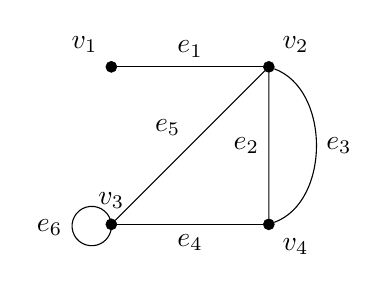
\begin{tikzpicture}[
	vertex/.style={ circle, draw, very thin, fill, inner sep=0pt, minimum size=4pt },
	vertexg/.style={ black!40!white, circle, draw, very thin, fill, inner sep=0pt, minimum size=4pt },
	vertexo/.style={ circle, draw, very thin, inner sep=0pt, minimum size=4pt }
]

\node at (0,0) (v3) [vertex,label=above:$v_3$] {};
\draw (v3) arc (5:355:0.25cm) node[left=0.5cm] {$e_6$} to (v3);
\node at (2,0) (v4) [vertex,label=below right:$v_4$] {};
\draw (v3) to node[below] {$e_4$} (v4);
\node at (2,2) (v2) [vertex,label=above right:$v_2$] {};
\draw (v2) to node[above left] {$e_5$} (v3);
\node at (0,2) (v1) [vertex,label=above left:$v_1$] {};
\draw (v2) to node[above] {$e_1$} (v1);
\draw (v4) to node[left] {$e_2$} (v2) to [out=-20,in=20] node[right] {$e_3$} (v4);

\end{tikzpicture}
